\documentclass[14pt]{extarticle}

\usepackage{fontspec}
\setmainfont{Times New Roman}

% размер полей
\usepackage{geometry}
\geometry{a4paper, top=2cm, bottom=2cm, right=1.5cm, left=3cm}

 %debugging
%\usepackage{showframe}

% полуторный интервал
\usepackage{setspace}
\onehalfspacing

% абзацный отступ
\setlength{\parindent}{1.25cm}

% выравнивание текста по ширине
\sloppy

% списки
\usepackage{calc} % арифметические операции с величинами
\usepackage{enumitem}
\setlist{
    nosep,
    leftmargin=0pt,
    itemindent=\parindent + \labelwidth - \labelsep,
}

% подписи к рисункам и таблицам
\usepackage{caption}
\renewcommand{\figurename}{Рисунок}
\renewcommand{\tablename}{Таблица}
\DeclareCaptionFormat{custom}
{
    \textit{#1#2#3}
}
\DeclareCaptionLabelSeparator{custom}{. }
\captionsetup{
    % хз какой это размер - 12 или нет, но выглядит меньше 14
    font=small,
    format=custom,
    labelsep=custom,
}

% картинки
\usepackage{graphicx}

% колонтитулы
\usepackage{fancyhdr}

% картинки и таблицы находятся именно в том месте текста где помещены (атрибут H)
\usepackage{float}

% таблицы
\usepackage{tabularray}

\graphicspath{ {6.3.2/models/} }
\begin{document}
\pagestyle{fancy}
\fancyhead{}
% disable header
\renewcommand{\headrulewidth}{0pt}
\fancyfoot[L]{Дубровских гр 221-361}
\fancyfoot[C]{ЛР 6.3.2}
\fancyfoot[R]{Продажа автотранспорта}
\singlespacing

\newpage
\begin{center}
    Министерство науки и высшего образования Российской Федерации
    Федеральное государственное автономное образовательное учреждение

    высшего образования

    \guillemotleft МОСКОВСКИЙ ПОЛИТЕХНИЧЕСКИЙ УНИВЕРСИТЕТ\guillemotright

    (МОСКОВСКИЙ ПОЛИТЕХ)
\end{center}
\noindent
\bigbreak
\bigbreak
\bigbreak
\bigbreak
\begin{center}
    ЛАБОРАТОРНАЯ РАБОТА 6.3.2

    По курсу Проектирования пользовательских интерфейсов в веб

    \textbf{Анализ цветовых палитр сайтов. Цвета в системе HEX}
    \bigbreak
    \bigbreak
    \bigbreak
    \bigbreak
    ТЕМА

    \guillemotleft\textbf{САЙТ ДЛЯ ПРОДАЖИ И ПОИСКА АВТОМОБИЛЕЙ}\guillemotright
\end{center}
\noindent
\bigbreak
\bigbreak
\bigbreak
\bigbreak
\bigbreak
\bigbreak
\bigbreak
\bigbreak
\bigbreak
\bigbreak
\hfill Выполнил

\hfill Дубровских Никита Евгеньевич

\hfill Группа 221-361
\bigbreak
\bigbreak
\bigbreak
\hfill Проверил

\hfill Натур ВВ
\vfill
\begin{center}
    Москва, 2024
\end{center}
\newpage
\onehalfspacing


\begin{center}
    \textbf{Лабораторная работа 6.3.2}

    \textbf{Анализ цветовых палитр сайтов. Цвета в системе HEX}
\end{center}

\textbf{Цель работы:} изучить цветовые аспекты проектирования интерфейс: стиль, мудборд, айдентику, теорию цвета и системы измерения цвета для веб.
\bigskip

\textbf{Задачи:}

\begin{enumerate}
    \item Познакомиться с основами теории цвета
    \item Рассмотреть системы измерения цвета и его кодирование для веб-продуктов
    \item Выбрать стиль веб-ресурса (сайта, веб-приложения)
    \item Проанализировать цветовые палитры пяти сайтов-аналогов (Ресурс Adobe Color позволяет применить правила гармонии цветов извлечь (извлечение темы) цветовую палитру из изображения сайта и мудборда). Определить вид их палитр.
    \item Определить айдентику сайтов пяти аналогов
\end{enumerate}
\bigskip

\textbf{Основные термины}

\begin{itemize}
    \item Теория цвета – наука о сочетании и взаимодействии цветов. Включает правила для гармоничного подбора цветовых комбинаций в дизайне, влияющие на восприятие сайта пользователями.
    \item HEX – система кодирования цвета, которая использует шестизначное шестнадцатеричное значение для обозначения каждого цвета, например \#FFFFFF для белого.
    \item Айдентика – совокупность уникальных визуальных и смысловых элементов бренда, включающих цветовую палитру, логотип, фирменный стиль, типографику и мудборд. Айдентика обеспечивает узнаваемость и ассоциативность бренда.
    \item Цветовая палитра – набор оттенков, подобранных для гармоничного сочетания, подчеркивающих стиль и настроение бренда. Используется для оформления интерфейса сайта и элементов призыва к действию (CTA).
    \item Психология цвета – область исследования влияния цвета на эмоции и поведение людей. Используется для улучшения взаимодействия пользователя с интерфейсом и повышения конверсии.
    \item Круг Иттена – цветовой круг, который помогает подбирать гармоничные цветовые сочетания.
\end{itemize}
\bigskip

\textbf{Выбор стиля сайта}

Стилем сайта выбран \guillemotleft Flat\guillemotright , так как:
\begin{itemize}
    \item предполагает минимальное использование декоративных элементов и сложных графических эффектов. Это делает интерфейс более чистым и понятным, что особенно важно для пользователей, которые ищут информацию о машинах. Простота в дизайне способствует лучшему восприятию контента и облегчает навигацию.
    \item акцентирует внимание на контенте, делая его более доступным. Четкие шрифты, яркие кнопки и контрастные цвета позволяют пользователям быстро находить нужные объявления, что критично для сайтов с большим количеством информации.
    \item хорошо подходит для адаптивных веб-сайтов. Он обеспечивает эффективное отображение на различных устройствах — от мобильных телефонов до десктопов. В условиях роста мобильного трафика важно, чтобы сайт был удобен для пользователей на любом устройстве.
    \item не требует использования тяжелых графических элементов и сложных эффектов, это может значительно снизить время загрузки страниц. Быстрая загрузка улучшает пользовательский опыт и влияет на SEO-оптимизацию.
    \item ассоциируется с современными тенденциями веб-дизайна и может помочь создать у пользователей ощущение, что сайт является актуальным и надежным. Это особенно важно для торговых платформ, где доверие играет ключевую роль.
    \item благодаря простоте структуры flat-дизайна, изменения и обновления на сайте можно вносить быстрее и легче. Это важно для платформ с динамическим контентом, таких как сайты объявлений.
    \item позволяет сосредоточиться на функциональности сайта, что помогает пользователям легко выполнять такие действия, как поиск, фильтрация и сортировка объявлений, без отвлечения на ненужные визуальные элементы.
\end{itemize}

\textbf{Определение цветовой палитры сайтов-аналогов}
\bigskip

\noindent
\begin{minipage}{\linewidth}
    \fbox{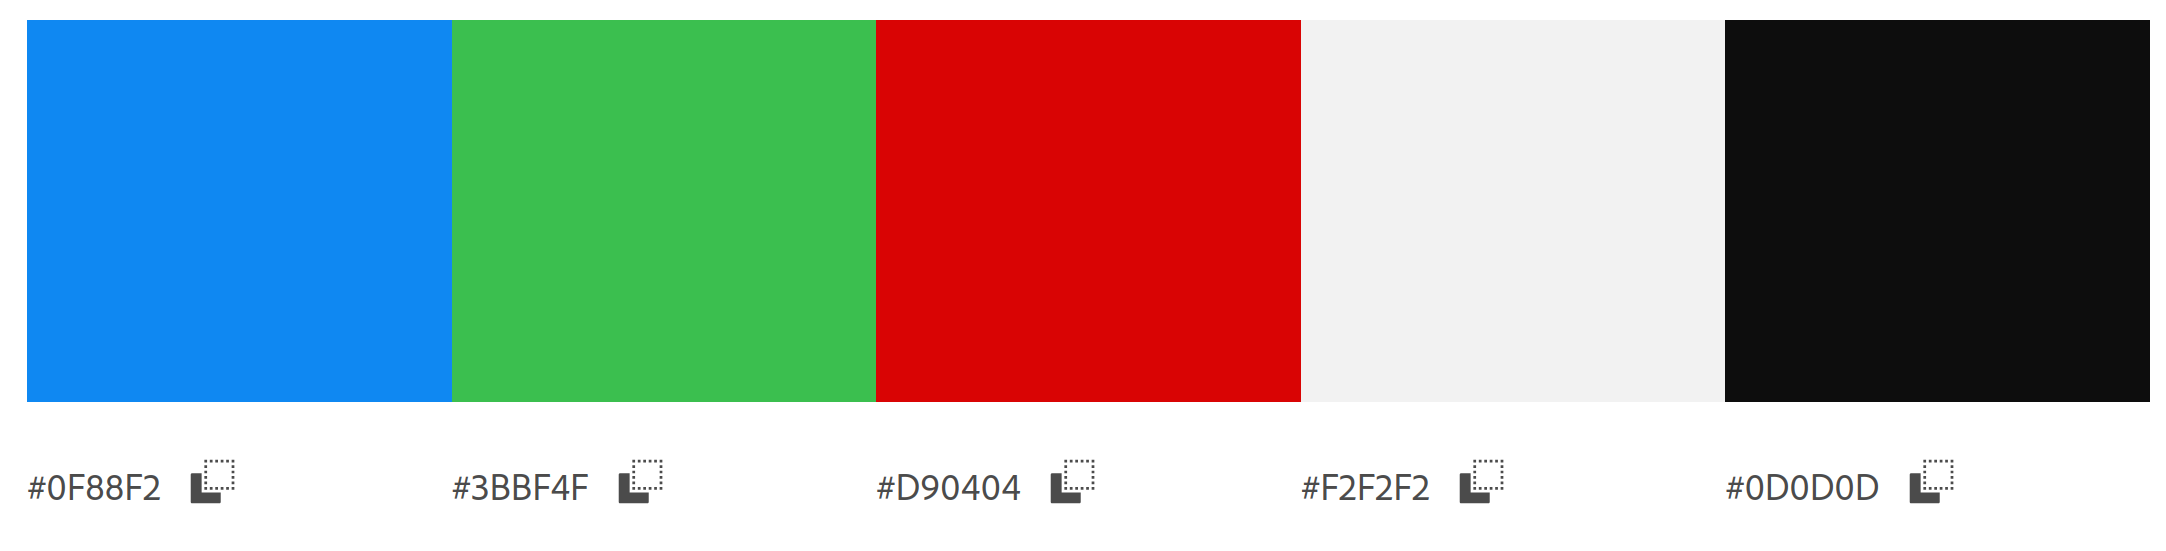
\includegraphics[width=\linewidth]{auto_ru}}
    \captionof{figure}{Палитра auto.ru}
\end{minipage}
\bigskip

\noindent
\begin{minipage}{\linewidth}
    \fbox{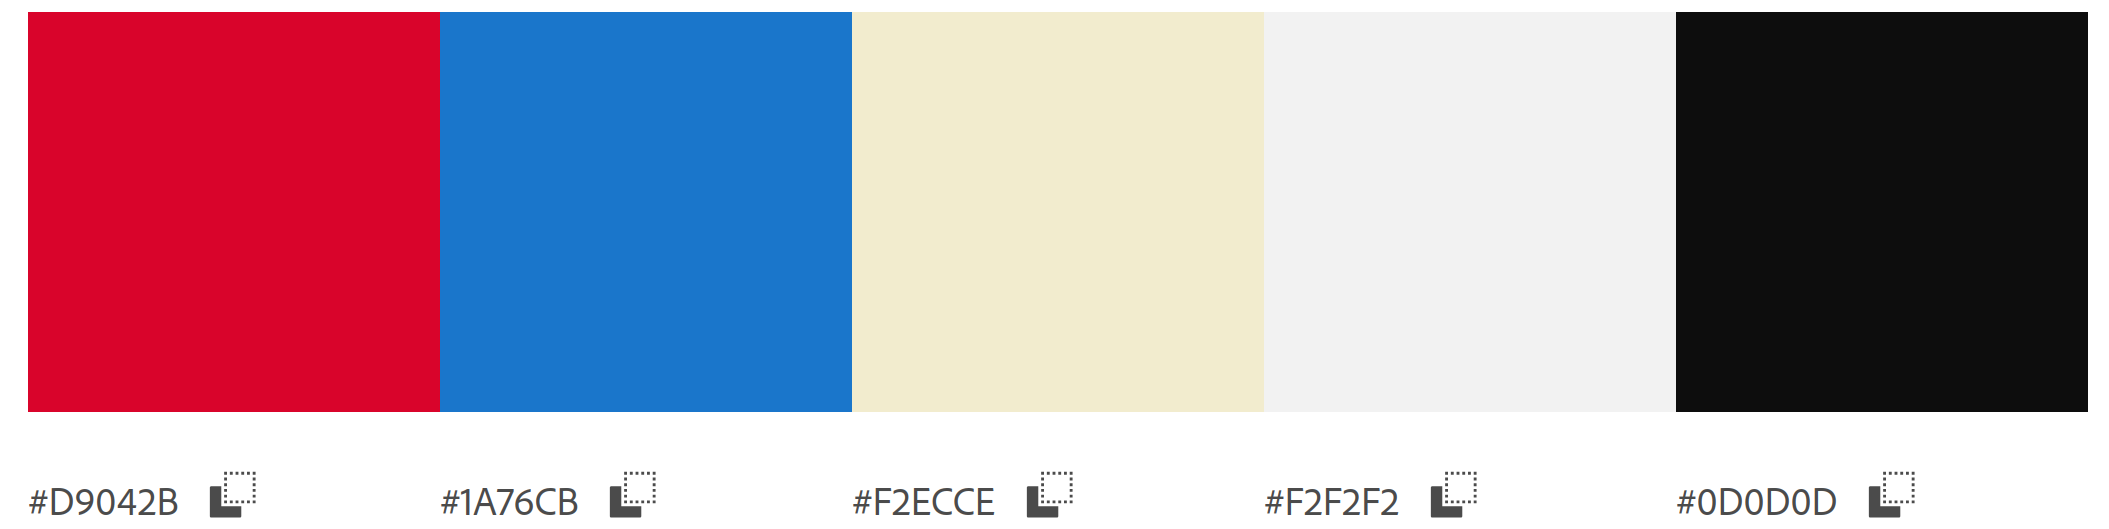
\includegraphics[width=\linewidth]{drom_ru_pallete}}
    \captionof{figure}{Палитра drom.ru}
\end{minipage}
\bigskip

\noindent
\begin{minipage}{\linewidth}
    \fbox{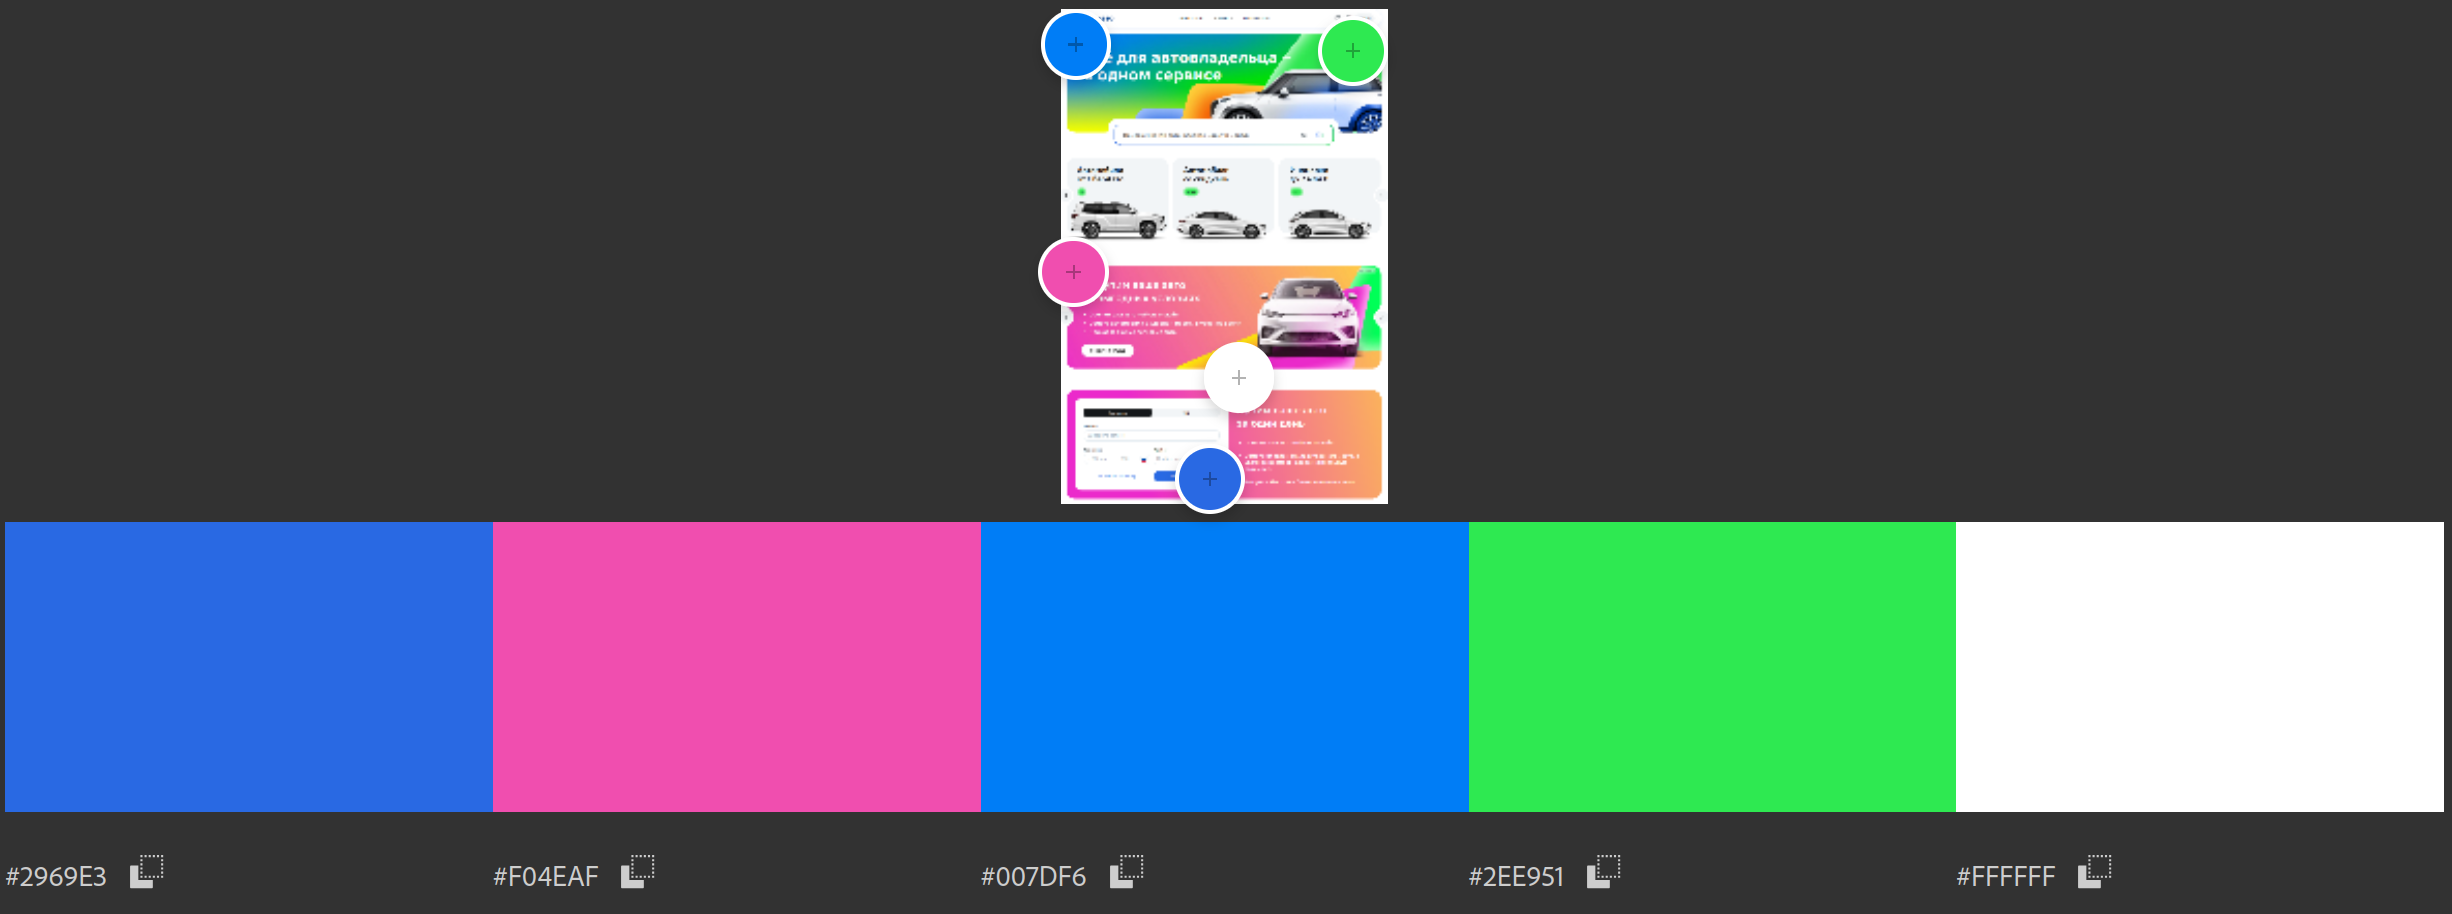
\includegraphics[width=\linewidth]{sberauto_com_pallete}}
    \captionof{figure}{Палитра sberauto.com}
\end{minipage}
\bigskip

\noindent
\begin{minipage}{\linewidth}
    \fbox{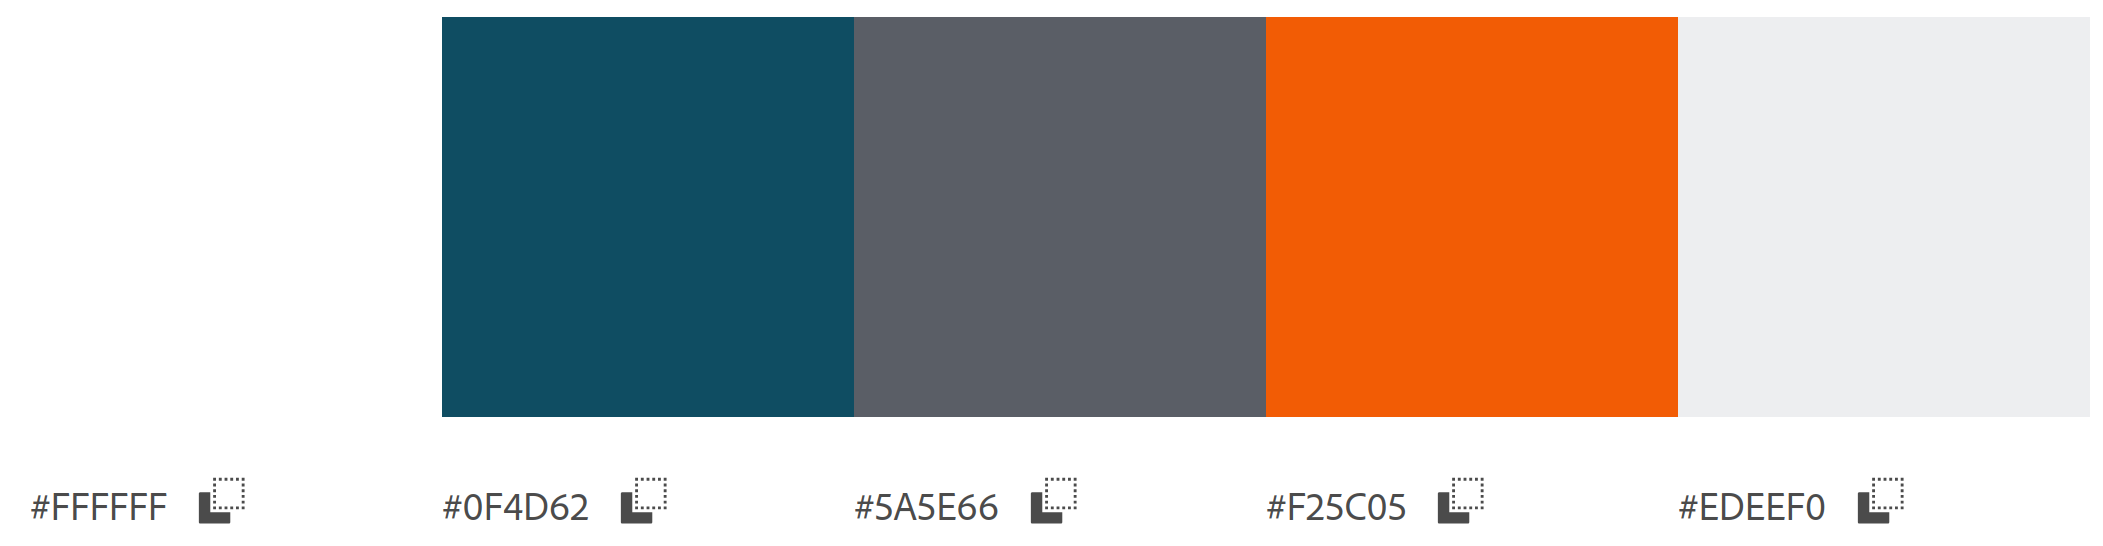
\includegraphics[width=\linewidth]{mobile_de_pallete}}
    \captionof{figure}{Палитра mobile.de}
\end{minipage}
\bigskip

\noindent
\begin{minipage}{\linewidth}
    \fbox{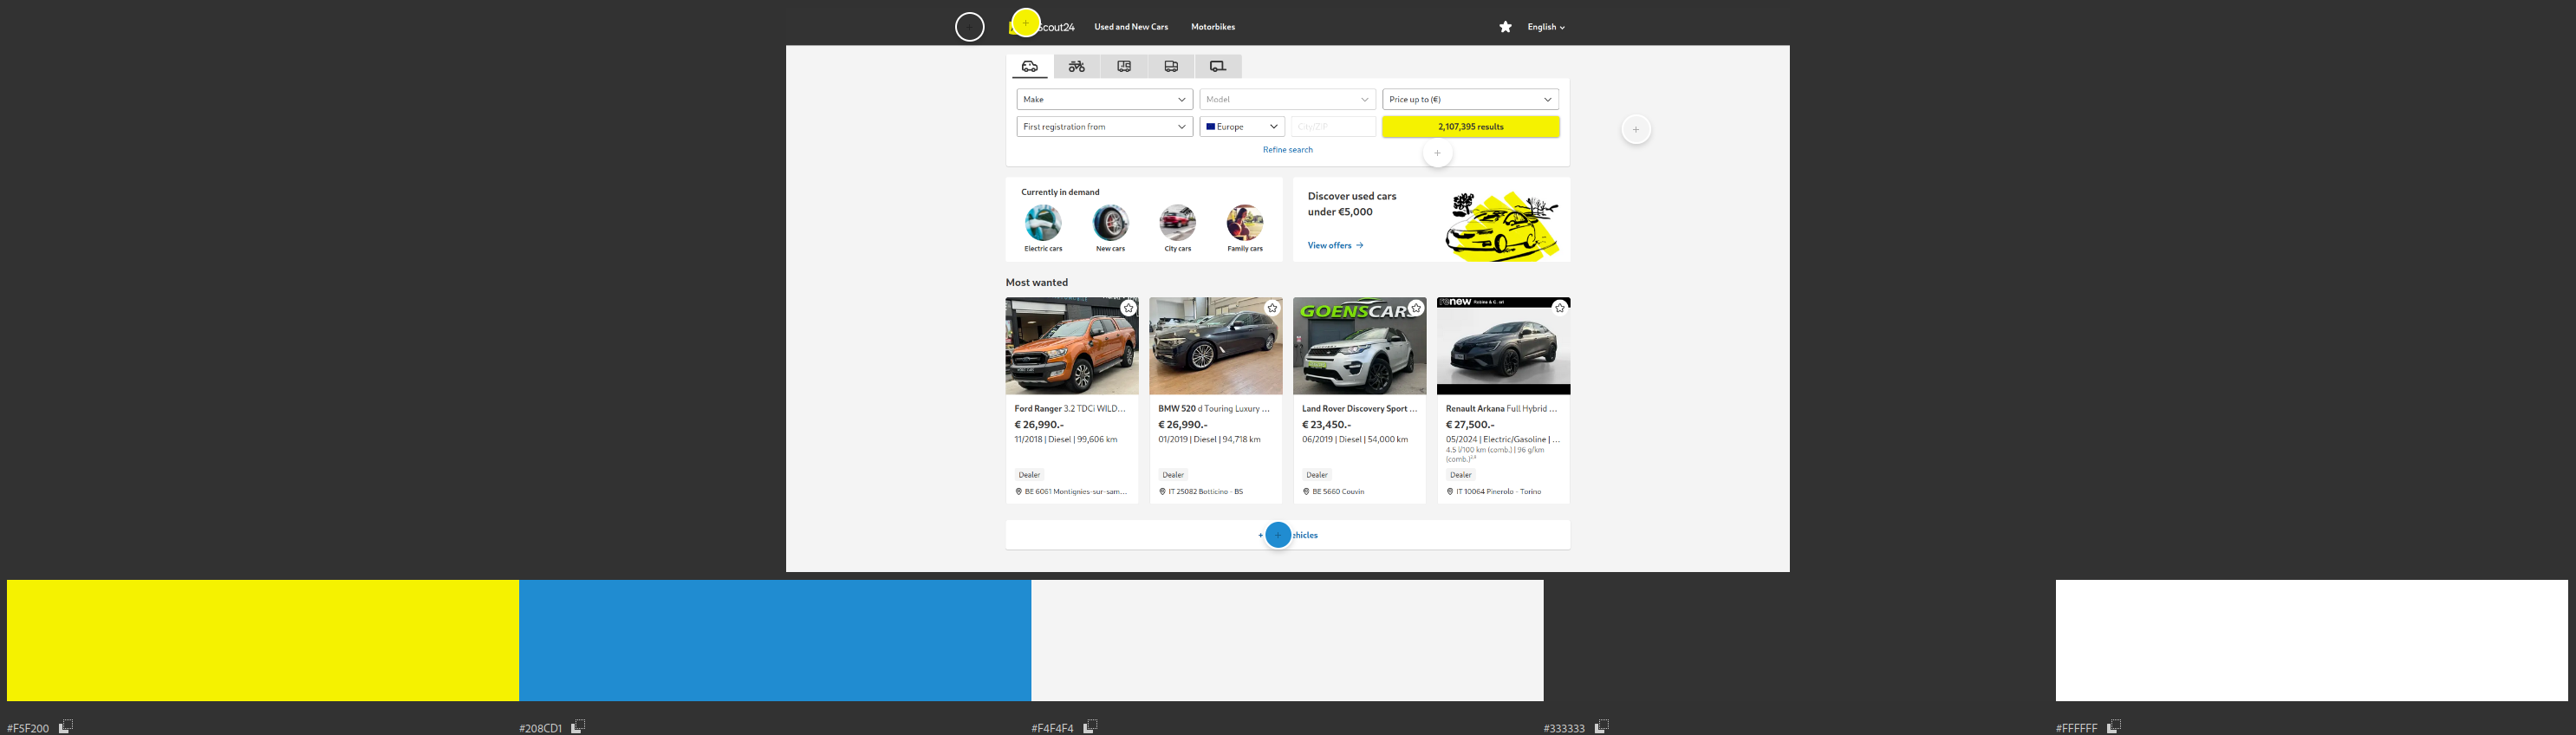
\includegraphics[width=\linewidth]{autoscout24_com_pallete}}
    \captionof{figure}{Палитра autoscout24.com}
\end{minipage}
\bigskip

\textbf{Логотипы сайтов-аналогов}
\bigskip

\noindent
\begin{minipage}{\linewidth}
    \fbox{
\includegraphics[width=\linewidth]{auto_logo}}
    \captionof{figure}{Логотип auto.ru}
\end{minipage}
\bigskip

\noindent
\begin{minipage}{\linewidth}
    \fbox{
\includegraphics[width=\linewidth]{drom_logo}}
    \captionof{figure}{Логотип drom.ru}
\end{minipage}
\bigskip

\noindent
\begin{minipage}{\linewidth}
    \fbox{
\includegraphics[width=\linewidth]{sberauto_logo}}
    \captionof{figure}{Логотип sberauto.com}
\end{minipage}
\bigskip

\noindent
\begin{minipage}{\linewidth}
    \fbox{
\includegraphics[width=\linewidth]{mobile_logo}}
    \captionof{figure}{Логотип mobile.de}
\end{minipage}
\bigskip
\noindent

\noindent
\begin{minipage}{\linewidth}
    \fbox{
\includegraphics[width=\linewidth]{autoscout_logo}}
    \captionof{figure}{Логотип autoscout24.com}
\end{minipage}
\bigskip

\textbf{Таблица айдентики сайтов-аналогов}
\bigskip

% \usepackage{tabularray}
\begin{table}[H]
    \captionsetup{justification=raggedright,singlelinecheck=false}
\caption{Таблица айдентики}
\centering
\begin{tblr}{
  width = \linewidth,
  colspec = {Q[302]Q[123]Q[494]},
  hlines,
  vlines,
}
Сайт                     & Стиль & Шрифт                     \\
\textit{auto.ru}         & Flat  & YS Text, YS Geo           \\
\textit{drom.ru}         & Flat  & Arial                     \\
\textit{sberauto.com}    & Flat  & SBSansText, SBSansDisplay \\
\textit{mobile.de}       & Flat  & Gibson                    \\
\textit{autoscout24.com} & Flat  & system-ui                 
\end{tblr}
\end{table}
\bigskip

\textbf{Контрольные вопросы и ответы}

\begin{enumerate}
    \item Чем определяется стилевое решение сайта?

    Стилевое решение сайта определяется целями и задачами проекта, а также предпочтениями целевой аудитории. Стиль сайта должен гармонично сочетать элементы дизайна, поддерживать контент и визуально передавать идею и концепцию бренда. Стилевое оформление способствует удобству навигации, создавая единый и запоминающийся интерфейс.
    \item Что такое айдентика?

    Айдентика – это набор визуальных и смысловых элементов, таких как логотип, цветовая палитра, фирменный стиль, типографика и мудборд, которые делают бренд узнаваемым и отличают его от конкурентов. Она помогает выразить ценности и основные идеи бренда, формируя целостный образ и ассоциации у целевой аудитории.
    \item Какие существуют рекомендации по количеству и соотношению основных цветов интерфейса?

    Рекомендуется использовать 3-4 основных цвета в интерфейсе: один доминирующий, один акцентный и один-два дополнительных. Доминирующий цвет занимает основное пространство, акцентный выделяет ключевые элементы (например, кнопки CTA), а дополнительные дополняют и поддерживают общий стиль.
    \item Какую роль играет психология цвета в интерфейсе?

    Психология цвета помогает создавать эмоциональные отклики и влияет на поведение пользователей. Правильный подбор цветов может привлечь внимание, укрепить доверие, подчеркнуть важность информации и повысить конверсию. Например, теплые цвета могут вызвать чувство энергии, а холодные — спокойствие и уверенность.
    \item Какие виды палитр известны? Их различия?

        Монохромная (оттенки одного цвета, создающие гармоничный и спокойный дизайн), комплементарная (сочетание противоположных на цветовом круге оттенков для контраста), аналогичная (соседние цвета на круге Иттена, создающие мягкие переходы), триадная (три цвета, расположенные равномерно на круге, для баланса и контраста).
    Различия этих палитр заключаются в уровне контраста и гармонии, создаваемом при их использовании.
    \item Как кодируется цвет для веб-ресурсов? Какое это имеет значение для дальнейших этапов разработки сайта?

    Цвет для веб-ресурсов кодируется в системах HEX, RGB и HSL. HEX используется наиболее часто, так как удобно отображает цвет в шестнадцатеричном формате (\#RRGGBB). RGB определяет цвет комбинацией красного, зеленого и синего (от 0 до 255), а HSL — тоном, насыщенностью и светлотой. Эти системы помогают разработчикам и дизайнерам точно передавать цветовую гамму на различных устройствах, обеспечивая согласованность бренда.
\end{enumerate}

\end{document}
